\documentclass[ignorenonframetext,]{beamer}
\setbeamertemplate{caption}[numbered]
\setbeamertemplate{caption label separator}{: }
\setbeamercolor{caption name}{fg=normal text.fg}
\beamertemplatenavigationsymbolsempty
\usepackage{lmodern}
\usepackage{amssymb,amsmath}
\usepackage{ifxetex,ifluatex}
\usepackage{fixltx2e} % provides \textsubscript
\ifnum 0\ifxetex 1\fi\ifluatex 1\fi=0 % if pdftex
  \usepackage[T1]{fontenc}
  \usepackage[utf8]{inputenc}
\else % if luatex or xelatex
  \ifxetex
    \usepackage{mathspec}
  \else
    \usepackage{fontspec}
  \fi
  \defaultfontfeatures{Ligatures=TeX,Scale=MatchLowercase}
\fi
\usetheme[]{Madrid}
\usecolortheme{whale}
% use upquote if available, for straight quotes in verbatim environments
\IfFileExists{upquote.sty}{\usepackage{upquote}}{}
% use microtype if available
\IfFileExists{microtype.sty}{%
\usepackage{microtype}
\UseMicrotypeSet[protrusion]{basicmath} % disable protrusion for tt fonts
}{}
\newif\ifbibliography
\hypersetup{
            pdftitle={Coding for Reproducible Research},
            pdfauthor={Luiza Andrade, Leonardo Viotti \& Rob Marty},
            pdfborder={0 0 0},
            breaklinks=true}
\urlstyle{same}  % don't use monospace font for urls
\usepackage{color}
\usepackage{fancyvrb}
\newcommand{\VerbBar}{|}
\newcommand{\VERB}{\Verb[commandchars=\\\{\}]}
\DefineVerbatimEnvironment{Highlighting}{Verbatim}{commandchars=\\\{\}}
% Add ',fontsize=\small' for more characters per line
\usepackage{framed}
\definecolor{shadecolor}{RGB}{248,248,248}
\newenvironment{Shaded}{\begin{snugshade}}{\end{snugshade}}
\newcommand{\KeywordTok}[1]{\textcolor[rgb]{0.13,0.29,0.53}{\textbf{#1}}}
\newcommand{\DataTypeTok}[1]{\textcolor[rgb]{0.13,0.29,0.53}{#1}}
\newcommand{\DecValTok}[1]{\textcolor[rgb]{0.00,0.00,0.81}{#1}}
\newcommand{\BaseNTok}[1]{\textcolor[rgb]{0.00,0.00,0.81}{#1}}
\newcommand{\FloatTok}[1]{\textcolor[rgb]{0.00,0.00,0.81}{#1}}
\newcommand{\ConstantTok}[1]{\textcolor[rgb]{0.00,0.00,0.00}{#1}}
\newcommand{\CharTok}[1]{\textcolor[rgb]{0.31,0.60,0.02}{#1}}
\newcommand{\SpecialCharTok}[1]{\textcolor[rgb]{0.00,0.00,0.00}{#1}}
\newcommand{\StringTok}[1]{\textcolor[rgb]{0.31,0.60,0.02}{#1}}
\newcommand{\VerbatimStringTok}[1]{\textcolor[rgb]{0.31,0.60,0.02}{#1}}
\newcommand{\SpecialStringTok}[1]{\textcolor[rgb]{0.31,0.60,0.02}{#1}}
\newcommand{\ImportTok}[1]{#1}
\newcommand{\CommentTok}[1]{\textcolor[rgb]{0.56,0.35,0.01}{\textit{#1}}}
\newcommand{\DocumentationTok}[1]{\textcolor[rgb]{0.56,0.35,0.01}{\textbf{\textit{#1}}}}
\newcommand{\AnnotationTok}[1]{\textcolor[rgb]{0.56,0.35,0.01}{\textbf{\textit{#1}}}}
\newcommand{\CommentVarTok}[1]{\textcolor[rgb]{0.56,0.35,0.01}{\textbf{\textit{#1}}}}
\newcommand{\OtherTok}[1]{\textcolor[rgb]{0.56,0.35,0.01}{#1}}
\newcommand{\FunctionTok}[1]{\textcolor[rgb]{0.00,0.00,0.00}{#1}}
\newcommand{\VariableTok}[1]{\textcolor[rgb]{0.00,0.00,0.00}{#1}}
\newcommand{\ControlFlowTok}[1]{\textcolor[rgb]{0.13,0.29,0.53}{\textbf{#1}}}
\newcommand{\OperatorTok}[1]{\textcolor[rgb]{0.81,0.36,0.00}{\textbf{#1}}}
\newcommand{\BuiltInTok}[1]{#1}
\newcommand{\ExtensionTok}[1]{#1}
\newcommand{\PreprocessorTok}[1]{\textcolor[rgb]{0.56,0.35,0.01}{\textit{#1}}}
\newcommand{\AttributeTok}[1]{\textcolor[rgb]{0.77,0.63,0.00}{#1}}
\newcommand{\RegionMarkerTok}[1]{#1}
\newcommand{\InformationTok}[1]{\textcolor[rgb]{0.56,0.35,0.01}{\textbf{\textit{#1}}}}
\newcommand{\WarningTok}[1]{\textcolor[rgb]{0.56,0.35,0.01}{\textbf{\textit{#1}}}}
\newcommand{\AlertTok}[1]{\textcolor[rgb]{0.94,0.16,0.16}{#1}}
\newcommand{\ErrorTok}[1]{\textcolor[rgb]{0.64,0.00,0.00}{\textbf{#1}}}
\newcommand{\NormalTok}[1]{#1}
\usepackage{graphicx,grffile}
\makeatletter
\def\maxwidth{\ifdim\Gin@nat@width>\linewidth\linewidth\else\Gin@nat@width\fi}
\def\maxheight{\ifdim\Gin@nat@height>\textheight0.8\textheight\else\Gin@nat@height\fi}
\makeatother
% Scale images if necessary, so that they will not overflow the page
% margins by default, and it is still possible to overwrite the defaults
% using explicit options in \includegraphics[width, height, ...]{}
\setkeys{Gin}{width=\maxwidth,height=\maxheight,keepaspectratio}

% Prevent slide breaks in the middle of a paragraph:
\widowpenalties 1 10000
\raggedbottom

\AtBeginPart{
  \let\insertpartnumber\relax
  \let\partname\relax
  \frame{\partpage}
}
\AtBeginSection{
  \ifbibliography
  \else
    \let\insertsectionnumber\relax
    \let\sectionname\relax
    \frame{\sectionpage}
  \fi
}
\AtBeginSubsection{
  \let\insertsubsectionnumber\relax
  \let\subsectionname\relax
  \frame{\subsectionpage}
}

\setlength{\parindent}{0pt}
\setlength{\parskip}{6pt plus 2pt minus 1pt}
\setlength{\emergencystretch}{3em}  % prevent overfull lines
\providecommand{\tightlist}{%
  \setlength{\itemsep}{0pt}\setlength{\parskip}{0pt}}
\setcounter{secnumdepth}{0}
\AtBeginSection[]
{
 \begin{frame}<beamer>
 \frametitle{Outline}
 \tableofcontents[currentsection]
 \end{frame}
}

\titlegraphic{
        \begin{figure}
        	\begin{minipage}[b]{0.3\textwidth}
            
\includegraphics[width=0.7\linewidth]{img/DIME_logo.png}
          \end{minipage}
          \hspace{1cm}
        	  \begin{minipage}[b]{0.3\textwidth}
            
\includegraphics[width=0.9\linewidth]{img/wbg.png}
            \vspace{0.5cm}
            \end{minipage}
        \end{figure}
        }

\usepackage{float}
\usepackage{adjustbox}
\usepackage{colortbl}
   
\definecolor{myColor}{rgb}{.05,.58,.71}
\usecolortheme[named=myColor]{structure}

\title{Coding for Reproducible Research}
\subtitle{R for Stata Users}
\author{Luiza Andrade, Leonardo Viotti \& Rob Marty}
\date{November-December 2018}

\begin{document}
\frame{\titlepage}

\begin{frame}
\tableofcontents[hideallsubsections]
\end{frame}

\section{Introduction}\label{introduction}

\begin{frame}{Why are we here today?}

\begin{block}{Code is a research output}

We often think of code as a mean to an end, but code is an end in
itself.

\end{block}

\end{frame}

\begin{frame}{Reproducibility}

\begin{block}{Can other people...}
      \begin{itemize}
        \item run your code?
      \item recreate your results?
      \item understand what you are doing and why?
      \item make changes to your code if necessary?
    \end{itemize}
  \end{block}

\end{frame}

\begin{frame}{Introduction}

\begin{block}{Objective}
      Create an R Master Script.
  \end{block}

\textbf{Content}

\begin{enumerate}
      \item Comments
      \item Using R Studio to create a code index
      \item Indenting
      \item File paths
      \item If statements
      \item Using functions within functions
      \item Packages
      \item Loops
    \end{enumerate}

\end{frame}

\begin{frame}[fragile]{Introduction}

\begin{itemize}
\tightlist
\item
  For the purpose of this training, we will assume that you are dealing
  with a specific folder structure
\item
  Folder organization, though an important part of data work, is outside
  the scope of this course
\item
  You can find resources about it in the appendix, and we have sent you
  a folder that is organized as we want it to be
\item
  To follow today's session, go to the \texttt{DataWork/Code} folder and
  open the file called
  \texttt{Lab\ 4\ -\ Coding\ for\ Reproducible\ Research.R}
\end{itemize}

\end{frame}

\begin{frame}{Master scripts}

\begin{itemize}
\tightlist
\item
  Just like in Stata, a Master script must be a map of all data work
\item
  It should be possible to follow all data work in the data folder, from
  raw data to analysis output, by following the master script
\item
  It should also be possible to run all the code for the project by
  simply running the Master script
\item
  Finally, in Stata, the Master Script is where you create globals. You
  can do the same in R by just creating new objects
\end{itemize}

\end{frame}

\section{Initial Settings}\label{initial-settings}

\begin{frame}[fragile]{Initial Settings}

A Stata do-file typically starts with a few settings:

\begin{verbatim}
    clear
    set maxvar 120000
    set more off
\end{verbatim}

\end{frame}

\begin{frame}[fragile]{Initial Settings}

\begin{itemize}
\tightlist
\item
  We don't need to set the memory or the maximum number of variables in
  R, and the equivalent of \texttt{more} is the default in R
\item
  However, if you saved the last RStudio session in \texttt{.Rhistory},
  the objects that were in RStudio's memory last time you closed it will
  still be there whenever you open it again
\item
  You can see all the objects currently in you memory in the
  \emph{Environment} pane
\end{itemize}

\end{frame}

\begin{frame}[fragile]{Initial Settings}

\begin{block}{Exercise 1: Clear workspace}

\begin{itemize}
\tightlist
\item
  Make sure the \texttt{Environment} window is open. Is anything there?
\item
  Create an object called \texttt{foo} with any content you pick
\item
  Type \texttt{ls()} to print the names of the object in memory
\item
  Type \texttt{rm(foo)} to remove the \texttt{foo} object from you
  memory
\item
  To remove all objects, use \texttt{rm(list=ls())}
\end{itemize}

\end{block}

\end{frame}

\begin{frame}{Initial Settings}

\begin{figure}
\centering
  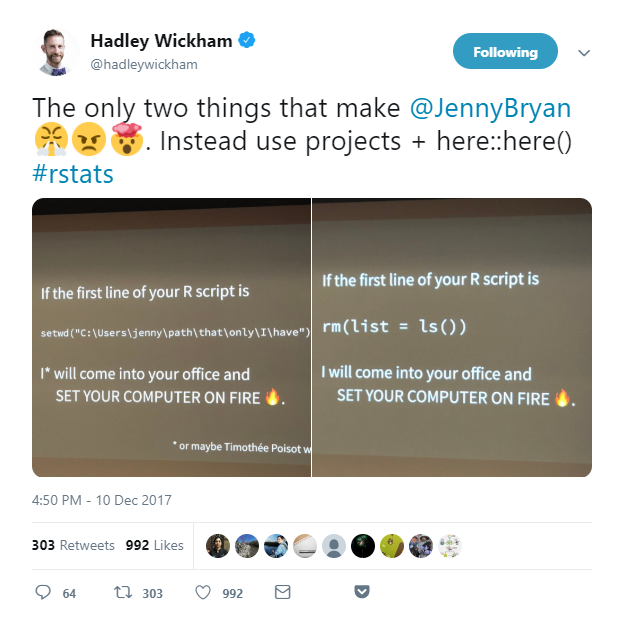
\includegraphics[width=12cm,height=7.7cm]{img/rm.png}
\end{figure}

\end{frame}

\begin{frame}{Initial Settings}

\begin{block}{Exercise 2: No one will burn your computer}

Here's how you change these settings

\end{block}

\end{frame}

\begin{frame}{Initial Settings}

\begin{figure}
\centering
  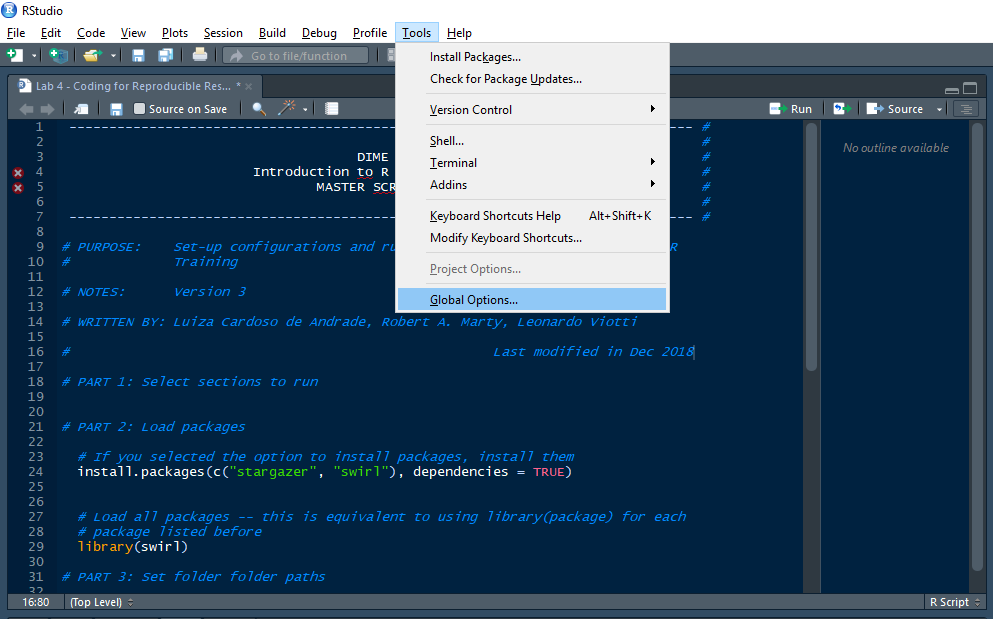
\includegraphics[width=12cm,height=7.7cm]{img/Options1.png}
\end{figure}

\end{frame}

\begin{frame}{Initial Settings}

\begin{figure}
\centering
  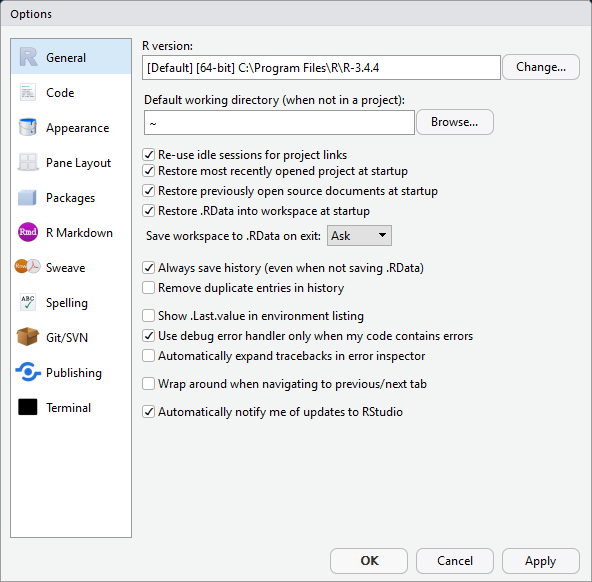
\includegraphics[width=12cm,height=7.7cm]{img/Options2.png}
\end{figure}

\end{frame}

\begin{frame}{Initial Settings}

\begin{figure}
\centering
  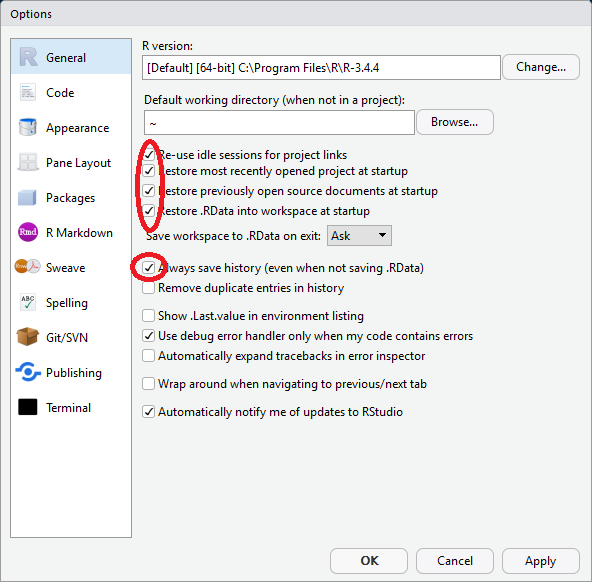
\includegraphics[width=12cm,height=7.7cm]{img/Options3.png}
\end{figure}

\end{frame}

\section{Commenting}\label{commenting}

\begin{frame}{Why comment?}

Comments have two purposes:

\begin{enumerate}
    \item Tell the reader what you are doing
    \item Tell the reader why you do what you do
  \end{enumerate}

If you have ever read code with no comments, you probably understand why
they are necessary.

\end{frame}

\begin{frame}{Commenting}

\begin{itemize}
    \item Let's take a look at the script we just opened
    \item You can see that the first few lines in the script are the header, but they're not commented out
    \item In R, errors will not always break your code, so you should still be able to run this script
    \item However, not commenting out comments is still bad practice, as it makes the code harder to read
  \end{itemize}

\end{frame}

\begin{frame}[fragile]{Commenting}

\begin{itemize}
\tightlist
\item
  To comment a line, write \texttt{\#} as its first character
\item
  You can also add \texttt{\#} half way through a line to comment
  whatever comes after it
\item
  In Stata, you can use \texttt{/*} and \texttt{*/} to comment part of a
  line's code. That is not possible in R: whatever comes after
  \texttt{\#} will be a comment
\item
  To comment a selection of lines, press \texttt{Ctrl\ +\ Shift\ +\ C}
\end{itemize}

\end{frame}

\begin{frame}{Commenting}

\begin{block}{Exercise 3: Commenting}

\begin{enumerate}
\def\labelenumi{\arabic{enumi}.}
\item
  Use the keyboard shortcut to comment the header of the script.
\item
  Use the keyboard shortcut to comment the header of the script again.
  What happened?
\end{enumerate}

\end{block}

\end{frame}

\section{Creating a document outline in
RStudio}\label{creating-a-document-outline-in-rstudio}

\begin{frame}[fragile]{Creating a document outline in RStudio}

\begin{itemize}
\tightlist
\item
  RStudio also allows you to create an interactive index for your
  scripts
\item
  To add a section to your code, create a commented line with the title
  of your section and add at least 4 trailing dashes, pound signs or
  equal signs after it
\end{itemize}

\begin{block}{Exercise 4: headers}

\begin{enumerate}
\def\labelenumi{\arabic{enumi}.}
\item
  Open the script index and make \texttt{PART\ 1} a section header. Do
  the same for parts 2 and 3.
\item
  Note that once you create a section header, an arrow appears right
  next to it. Click on the arrows of parts 2 and 3 to see what happens.
\end{enumerate}

\end{block}

\end{frame}

\begin{frame}[fragile]{Creating a document outline in RStudio}

\begin{itemize}
\tightlist
\item
  The outline can be accessed by clicking on the button on the top right
  corner of the script window. You can use it to jump from one section
  to another
\item
  You can also use the keyboard shortcuts \texttt{Alt\ +\ L}
  (\texttt{Cmd\ +\ Option\ +\ L} on Mac) and
  \texttt{Alt\ +\ Shift\ +\ L} to collapse and expand sections
\end{itemize}

\end{frame}

\section{Using packages}\label{using-packages}

\begin{frame}{Using packages}

\begin{itemize}
\tightlist
\item
  Since there is a lot of people developing for R, it can have many
  different functionalities
\item
  To make it simpler, these functionalities are bundled into packages
\item
  A package is the fundamental unit of shareable code
\item
  It may contain new functions, but also more complex functionalities,
  such as a Graphic User Interface (GUI) or settings for parallel
  processing (similar to Stata MP)
\item
  They can be shared through R's official repository - CRAN (10,000+
  packages reviewed and tested) and many other online sources
\item
  There are many other online sources such as Github, but it's important
  to be careful, as these probably haven't gone through a review process
  as rigorous as those in CRAN
\end{itemize}

\end{frame}

\begin{frame}[fragile]{Using packages}

\begin{itemize}
\tightlist
\item
  To install and use packages you can either do it with the user
  interface or by the command prompt.
\end{itemize}

\begin{Shaded}
\begin{Highlighting}[]
\CommentTok{# Installing a package}
\KeywordTok{install.packages}\NormalTok{(}\StringTok{"stargazer"}\NormalTok{,}
                 \DataTypeTok{dependencies =}\NormalTok{ T)}
\CommentTok{# the dependencies argument also installs all other packages}
\CommentTok{# that it may depend upon}
\end{Highlighting}
\end{Shaded}

\begin{itemize}
\tightlist
\item
  You only have to install a package once, but you have to load it every
  new session. To load a package type:
\end{itemize}

\begin{Shaded}
\begin{Highlighting}[]
\KeywordTok{library}\NormalTok{(stargazer)}
\end{Highlighting}
\end{Shaded}

\end{frame}

\begin{frame}{Using packages}

Once a package is loaded, you can use its features and functions. Here's
a list of some useful and cool packages:

\begin{itemize}
\tightlist
\item
  Rcmdr - Easy to use GUI
\item
  swirl - An interactive learning environment for R and statistics.
\item
  ggplot2 - beautiful and versatile graphics (the syntax is a pain,
  though)
\item
  stargazer - awesome latex regression and summary statistics tables
\item
  foreign - reads dtas and other formats from inferior statistical
  software
\item
  zoo - time series and panel data manipulation useful functions
\item
  data.table - some functions to deal with huge data sets
\item
  sp and rgeos - spatial analysis
\item
  multiwayvcov and sandwich - clustered and robust standard errors
\item
  RODBC, RMySQL, RPostgresSQL, RSQLite - For relational databases and
  using SQL in R.
\end{itemize}

\end{frame}

\begin{frame}[fragile]{Using packages}

\begin{block}{Exercise 5: Installing packages}

Install the \texttt{swirl} and \texttt{stargazer} packages, including
packages necessary for them to run.

\end{block}

\end{frame}

\begin{frame}[fragile]{Using packages}

\scriptsize

\begin{Shaded}
\begin{Highlighting}[]
  \CommentTok{# Install stargazer and swirl}
  \KeywordTok{install.packages}\NormalTok{(}\KeywordTok{c}\NormalTok{(}\StringTok{"stargazer"}\NormalTok{, }\StringTok{"swirl"}\NormalTok{), }\DataTypeTok{dependencies =} \OtherTok{TRUE}\NormalTok{)}
\end{Highlighting}
\end{Shaded}

\end{frame}

\section{Functions inception}\label{functions-inception}

\begin{frame}[fragile]{Functions inception}

\begin{itemize}
\tightlist
\item
  In R, you can use the output of one function as the input of another,
  as long as they have the same format
\item
  In fact, that's exactly what we just did when installing the packages
\item
  To see that, select just the first argument of the
  \texttt{install.packages} function and press \texttt{Ctrl\ +\ Enter}
\item
  The \texttt{c()} function, as we know, creates a vector with its
  arguments
\end{itemize}

\begin{Shaded}
\begin{Highlighting}[]
  \KeywordTok{c}\NormalTok{(}\StringTok{"stargazer"}\NormalTok{, }\StringTok{"swirl"}\NormalTok{)}
\end{Highlighting}
\end{Shaded}

\begin{verbatim}
## [1] "stargazer" "swirl"
\end{verbatim}

\end{frame}

\begin{frame}[fragile]{Functions inception}

\begin{itemize}
\tightlist
\item
  The resulting vector is used as an input to the
  \texttt{install.packages} function
\item
  We could also have stored this vector in the memory as an object and
  used that object as the input
\item
  In fact, that's exactly what we are going to do next, so the code
  doesn't get too polluted as we add new packages
\end{itemize}

\end{frame}

\begin{frame}[fragile]{Functions inception}

\begin{Shaded}
\begin{Highlighting}[]
  \CommentTok{# Create packages object}
\NormalTok{  packages <-}\StringTok{ }\KeywordTok{c}\NormalTok{(}\StringTok{"stargazer"}\NormalTok{,}
                \StringTok{"swirl"}\NormalTok{)}

  \CommentTok{# Use it as an input to the install.packageS() function}
  \KeywordTok{install.packages}\NormalTok{(packages,}
                   \DataTypeTok{dependencies =} \OtherTok{TRUE}\NormalTok{)}
\end{Highlighting}
\end{Shaded}

\end{frame}

\begin{frame}[fragile]{Using packages}

\begin{block}{Exercise 6: Load packages}

Load the packages you just installed, as well as the other packages used
in previous sessions.

\begin{itemize}
\tightlist
\item
  Note that the \texttt{library} function only accepts one argument.
  This means that you cannot use function inception with the
  \texttt{packages} object here, as its output format does not match the
  function input. In fact, you will need to load each of them
  separately.
\end{itemize}

\end{block}

\end{frame}

\begin{frame}[fragile]{Using packages}

\begin{Shaded}
\begin{Highlighting}[]
  \KeywordTok{library}\NormalTok{(swirl)}
  \KeywordTok{library}\NormalTok{(stargazer)}
  \KeywordTok{library}\NormalTok{(tidyverse)}
  \KeywordTok{library}\NormalTok{(openxlsx)}
  \KeywordTok{library}\NormalTok{(ggplot2)}
  \KeywordTok{library}\NormalTok{(plotly)}
\end{Highlighting}
\end{Shaded}

\end{frame}

\section{Looping}\label{looping}

\begin{frame}[fragile]{Looping}

\begin{itemize}
\tightlist
\item
  If you're thinking what happens as I add more packages here, you're
  going in the right direction
\item
  Repetition makes the code harder to read and to maintain
\end{itemize}

\begin{Shaded}
\begin{Highlighting}[]
    \CommentTok{# The DRY rule:}
\NormalTok{    DONT REPEAT YOURSELF}
\end{Highlighting}
\end{Shaded}

\end{frame}

\begin{frame}[fragile]{Looping}

\begin{itemize}
\tightlist
\item
  In Stata, we'd usually use a \texttt{foreach} loop to go through a
  list of objects
\item
  If you are a Stata coder, you are probably thinking of writing
  something like
\end{itemize}

\begin{verbatim}
  * Looping through packages
  foreach package in  swirl stargazer tidyverse ///
                      openxlsx ggplot2 plotly {
    library `package'
  }
\end{verbatim}

\end{frame}

\begin{frame}[fragile]{Looping}

\begin{itemize}
\tightlist
\item
  The equivalent to that in R would be to write a for loop like this
  (this code won't run, so don't try it yet)
\end{itemize}

\begin{Shaded}
\begin{Highlighting}[]
    \CommentTok{# A for loop in R}
    \ControlFlowTok{for}\NormalTok{ (package }\ControlFlowTok{in}\NormalTok{ packages) \{}
        \KeywordTok{library}\NormalTok{(package)}
\NormalTok{    \}}
\end{Highlighting}
\end{Shaded}

\end{frame}

\begin{frame}[fragile]{Looping}

\begin{itemize}
\tightlist
\item
  R, however, has a whole function family that allows users to loop
  through an object in a more efficient way
\item
  They're called \texttt{apply} and there are many of them, with
  different use cases
\item
  If you look for the \texttt{apply} help file, you can see all of them
\item
  For the purpose of this training, we will only use two of them,
  \texttt{sapply} and \texttt{apply}
\end{itemize}

\end{frame}

\begin{frame}[fragile]{Looping}

\begin{itemize}
\tightlist
\item
  \texttt{sapply(X,\ FUN,\ ...)}: applies a function to all elements of
  a vector or list and returns the result in a vector. Its arguments are

  \begin{itemize}
  \tightlist
  \item
    \textbf{X:} a matrix (or data frame) the function will be applied to
  \item
    \textbf{FUN:} the function you want to apply
  \item
    \textbf{\ldots{}:} possible function options
  \end{itemize}
\end{itemize}

\end{frame}

\begin{frame}[fragile]{Looping}

\begin{Shaded}
\begin{Highlighting}[]
    \CommentTok{# A for loop in R}
    \ControlFlowTok{for}\NormalTok{ (number }\ControlFlowTok{in} \KeywordTok{c}\NormalTok{(}\FloatTok{1.2}\NormalTok{,}\FloatTok{2.5}\NormalTok{)) \{}
      \KeywordTok{print}\NormalTok{(}\KeywordTok{round}\NormalTok{(number))}
\NormalTok{    \}}
\end{Highlighting}
\end{Shaded}

\begin{verbatim}
## [1] 1
## [1] 2
\end{verbatim}

\begin{Shaded}
\begin{Highlighting}[]
    \CommentTok{# A much more elegant loop in R}
    \KeywordTok{sapply}\NormalTok{(}\KeywordTok{c}\NormalTok{(}\FloatTok{1.2}\NormalTok{,}\FloatTok{2.5}\NormalTok{), round)}
\end{Highlighting}
\end{Shaded}

\begin{verbatim}
## [1] 1 2
\end{verbatim}

\end{frame}

\begin{frame}[fragile]{Looping}

\begin{block}{Exercise 7: Looping in R}

Use the \texttt{sapply()} function to apply the \texttt{library()}
function to all packages you have selected.

\begin{itemize}
\tightlist
\item
  TIP: to do this without creating errors, you will need to use that
  \texttt{...} argument and make the \texttt{character.only} argument of
  the \texttt{library()} function equal to \texttt{TRUE}
\end{itemize}

\end{block}

\end{frame}

\begin{frame}[fragile]{Looping}

\begin{Shaded}
\begin{Highlighting}[]
    \CommentTok{# Load all listed packages}
    \KeywordTok{sapply}\NormalTok{(packages, library, }\DataTypeTok{character.only =} \OtherTok{TRUE}\NormalTok{)}
\end{Highlighting}
\end{Shaded}

\end{frame}

\begin{frame}[fragile]{Looping}

A more general version is the \texttt{apply} function.

\begin{itemize}
\tightlist
\item
  \texttt{apply(X,\ MARGIN,\ FUN,\ ...)}: applies a function to all
  columns or rows of matrix. Its arguments are

  \begin{itemize}
  \tightlist
  \item
    \textbf{X:} a matrix (or data frame) the function will be applied to
  \item
    \textbf{MARGIN:} 1 to apply the function to all rows or 2 to apply
    the function to all columns
  \item
    \textbf{FUN:} the function you want to apply
  \item
    \textbf{\ldots{}:} possible function options
  \end{itemize}
\end{itemize}

\end{frame}

\begin{frame}[fragile]{Looping}

\begin{Shaded}
\begin{Highlighting}[]
    \CommentTok{# Create a matrix}
\NormalTok{    matrix <-}\StringTok{ }\KeywordTok{matrix}\NormalTok{(}\KeywordTok{c}\NormalTok{(}\DecValTok{1}\NormalTok{, }\DecValTok{24}\NormalTok{, }\DecValTok{9}\NormalTok{, }\DecValTok{6}\NormalTok{, }\DecValTok{9}\NormalTok{, }\DecValTok{4}\NormalTok{, }\DecValTok{2}\NormalTok{, }\DecValTok{74}\NormalTok{, }\DecValTok{2}\NormalTok{),}
                       \DataTypeTok{nrow =} \DecValTok{3}\NormalTok{)}

    \CommentTok{# Look at the matrix}
\NormalTok{    matrix}
\end{Highlighting}
\end{Shaded}

\begin{verbatim}
##      [,1] [,2] [,3]
## [1,]    1    6    2
## [2,]   24    9   74
## [3,]    9    4    2
\end{verbatim}

\end{frame}

\begin{frame}[fragile]{Looping}

\begin{Shaded}
\begin{Highlighting}[]
    \CommentTok{# Row means}
    \KeywordTok{apply}\NormalTok{(matrix, }\DecValTok{1}\NormalTok{, mean)}
\end{Highlighting}
\end{Shaded}

\begin{verbatim}
## [1]  3.00000 35.66667  5.00000
\end{verbatim}

\begin{Shaded}
\begin{Highlighting}[]
    \CommentTok{# Column means}
    \KeywordTok{apply}\NormalTok{(matrix, }\DecValTok{2}\NormalTok{, mean)}
\end{Highlighting}
\end{Shaded}

\begin{verbatim}
## [1] 11.333333  6.333333 26.000000
\end{verbatim}

\end{frame}

\begin{frame}[fragile]{Looping}

\begin{itemize}
\tightlist
\item
  The \texttt{apply()} function is a very powerful tool in R programming
\item
  To explore it to its full potential, we combine it with customized
  functions
\item
  This is beyond today's session, and we will come back to it in our
  last day, but you can give it a try on this session's assignment
\end{itemize}

\end{frame}

\section{Indentation}\label{indentation}

\begin{frame}[fragile]{Why indent?}

\scriptsize

\begin{Shaded}
\begin{Highlighting}[]
\CommentTok{# Here's some code}
\NormalTok{annualHappy_reg <-}\StringTok{ }\KeywordTok{aggregate}\NormalTok{(happy_score }\OperatorTok{~}\StringTok{ }\NormalTok{year }\OperatorTok{+}\StringTok{ }\NormalTok{region, }\DataTypeTok{data =}\NormalTok{ whr, }\DataTypeTok{FUN =}\NormalTok{ mean)}
\NormalTok{plot <-}\StringTok{ }\KeywordTok{ggplot}\NormalTok{(annualHappy_reg,}\KeywordTok{aes}\NormalTok{(}\DataTypeTok{y =}\NormalTok{ happy_score,}\DataTypeTok{x =}\NormalTok{ year, }\DataTypeTok{color =}\NormalTok{ region, }
\DataTypeTok{group =}\NormalTok{ region)) }\OperatorTok{+}\StringTok{ }\KeywordTok{geom_line}\NormalTok{() }\OperatorTok{+}\StringTok{ }\KeywordTok{geom_point}\NormalTok{()}
\KeywordTok{print}\NormalTok{(plot)}
\end{Highlighting}
\end{Shaded}

\end{frame}

\begin{frame}{Why indent?}

\includegraphics{Lab_4_-_Coding_for_Reproducible_Research_files/figure-beamer/unnamed-chunk-18-1.pdf}

\end{frame}

\begin{frame}[fragile]{Why indent?}

\begin{Shaded}
\begin{Highlighting}[]
\CommentTok{# Here's the same code}
\NormalTok{annualHappy_reg <-}\StringTok{ }
\StringTok{  }\KeywordTok{aggregate}\NormalTok{(happy_score }\OperatorTok{~}\StringTok{ }\NormalTok{year }\OperatorTok{+}\StringTok{ }\NormalTok{region,}
            \DataTypeTok{data =}\NormalTok{ whr,}
            \DataTypeTok{FUN =}\NormalTok{ mean)}

\NormalTok{plot <-}\StringTok{  }
\StringTok{  }\KeywordTok{ggplot}\NormalTok{(annualHappy_reg,}
         \KeywordTok{aes}\NormalTok{(}\DataTypeTok{y =}\NormalTok{ happy_score,}
             \DataTypeTok{x =}\NormalTok{ year, }
             \DataTypeTok{color =}\NormalTok{ region, }
             \DataTypeTok{group =}\NormalTok{ region)) }\OperatorTok{+}
\StringTok{  }\KeywordTok{geom_line}\NormalTok{() }\OperatorTok{+}\StringTok{ }
\StringTok{  }\KeywordTok{geom_point}\NormalTok{()}

\KeywordTok{print}\NormalTok{(plot)}
\end{Highlighting}
\end{Shaded}

\end{frame}

\begin{frame}{Why indent?}

\includegraphics{Lab_4_-_Coding_for_Reproducible_Research_files/figure-beamer/unnamed-chunk-20-1.pdf}

\end{frame}

\begin{frame}{Why indent?}

\begin{itemize}
\tightlist
\item
  Even though R understands what unindented code says, it can be quite
  difficult for a human being to read it
\item
  On the other hand, white space does not have a special meaning for R,
  so it will understand code that is more readable for a human being
\end{itemize}

\end{frame}

\begin{frame}{Indentation}

\begin{itemize}
    \item Indentation in R looks different than in Stata:
    \begin{itemize}
      \item To indent a whole line, you can select that line and press \texttt{Tab}
      \item To unindent a whole line, you can select that line and press \texttt{Shift + Tab}
      \item However, this will not always work for different parts of a code in the same line
    \end{itemize}
    \item In R, we typically don't introduce white space manually
    \item It's rather introduced by RStudio for us
  \end{itemize}

\end{frame}

\begin{frame}[fragile]{Indentation}

\begin{block}{Exercise 8: Indentation in R}

To see an example of how indenting works in RStudio, go back to our
first example with \texttt{sapply}:

\begin{Shaded}
\begin{Highlighting}[]
\CommentTok{# A much more elegant loop in R}
\KeywordTok{sapply}\NormalTok{(}\KeywordTok{c}\NormalTok{(}\FloatTok{1.2}\NormalTok{,}\FloatTok{2.5}\NormalTok{), round)}
\end{Highlighting}
\end{Shaded}

\begin{enumerate}
\def\labelenumi{\arabic{enumi}.}
\item
  Add a line between the two arguments of the function (the vector of
  numbers and the round function)
\item
  Now add a line between the numbers in the vector.
\end{enumerate}

\end{block}

\end{frame}

\begin{frame}[fragile]{Indentation}

Note that RStudio formats the different arguments of the function
differently:

\begin{Shaded}
\begin{Highlighting}[]
\CommentTok{# A much more elegant loop in R}
\KeywordTok{sapply}\NormalTok{(}\KeywordTok{c}\NormalTok{(}\FloatTok{1.2}\NormalTok{,}
         \FloatTok{2.5}\NormalTok{),}
\NormalTok{       round)}
\end{Highlighting}
\end{Shaded}

\end{frame}

\section{If statements}\label{if-statements}

\begin{frame}{If statements}

\begin{itemize}
\tightlist
\item
  Now, installing packages can be time-consuming, especially as the
  number of packages you're using grows, and each package only needs to
  be installed once
\item
  What can we bring from our Stata Master do-files to avoid installing
  packages twice?
\end{itemize}

\end{frame}

\begin{frame}{If statements}

\begin{itemize}
\tightlist
\item
  In Stata, section switches would be saved as locals
\item
  In R, the equivalent to that would be to create a new object
\end{itemize}

\begin{block}{Exercise 9: Creating an if statement}

Create a dummy scalar object called PACKAGES.

\begin{itemize}
\tightlist
\item
  TIP: Section switches can also be Boolean objects.
\end{itemize}

\end{block}

\end{frame}

\begin{frame}[fragile]{If statements}

\begin{itemize}
\tightlist
\item
  Now we need to create an if statement using this switch
\item
  If statements in R look like this:
\end{itemize}

\begin{Shaded}
\begin{Highlighting}[]
    \CommentTok{# Turn switch on}
\NormalTok{    PACKAGES <-}\StringTok{ }\DecValTok{1}

    \CommentTok{# Install packages}
    \ControlFlowTok{if}\NormalTok{ (PACKAGES }\OperatorTok{==}\StringTok{ }\DecValTok{1}\NormalTok{) \{}
      \KeywordTok{install.packages}\NormalTok{(packages,}
                       \DataTypeTok{dependencies =} \OtherTok{TRUE}\NormalTok{)}
\NormalTok{    \}}
\end{Highlighting}
\end{Shaded}

\end{frame}

\begin{frame}[fragile]{If statements}

\begin{itemize}
\tightlist
\item
  Possible variations would include
\end{itemize}

\begin{Shaded}
\begin{Highlighting}[]
    \CommentTok{# Turn switch on}
\NormalTok{    PACKAGES <-}\StringTok{ }\OtherTok{TRUE}

    \CommentTok{# Using a Boolean object}
    \ControlFlowTok{if}\NormalTok{ (PACKAGES }\OperatorTok{==}\StringTok{ }\OtherTok{TRUE}\NormalTok{) \{}
      \KeywordTok{install.packages}\NormalTok{(packages, }\DataTypeTok{dep =}\NormalTok{ T)}
\NormalTok{    \}}

    \CommentTok{# Which is the same as}
    \ControlFlowTok{if}\NormalTok{ (PACKAGES) \{}
      \KeywordTok{install.packages}\NormalTok{(packages, }\DataTypeTok{dep =}\NormalTok{ T)}
\NormalTok{    \}}
\end{Highlighting}
\end{Shaded}

\end{frame}

\section{File paths}\label{file-paths}

\begin{frame}{File paths}

\begin{itemize}
\tightlist
\item
  The next important part of a Master script are file paths
\item
  We recommend always using \textbf{explicit} and \textbf{dynamic} file
  paths
\end{itemize}

\end{frame}

\begin{frame}[fragile]{File paths}

\begin{itemize}
\tightlist
\item
  Implicit and static file path:
\end{itemize}

\begin{Shaded}
\begin{Highlighting}[]
  \CommentTok{# Set working directory}
  \KeywordTok{setwd}\NormalTok{(}\StringTok{"C:/Users/luiza/Documents/GitHub/dime-r-training/}
\StringTok{        DataWork/DataSets/Final"}\NormalTok{)}
  
  \CommentTok{# Load data set}
  \KeywordTok{read.csv}\NormalTok{(}\StringTok{"whr_panel.csv"}\NormalTok{,}
            \DataTypeTok{header =}\NormalTok{ T)}
\end{Highlighting}
\end{Shaded}

\end{frame}

\begin{frame}[fragile]{File paths}

\begin{itemize}
\tightlist
\item
  Explicit and static file path:
\end{itemize}

\begin{Shaded}
\begin{Highlighting}[]
  \CommentTok{# Load data set}
  \KeywordTok{read.csv}\NormalTok{(}\StringTok{"C:/Users/luiza/Documents/GitHub/dime-r-training/}
\StringTok{           DataWork/DataSets/Final/whr_panel.csv"}\NormalTok{,}
            \DataTypeTok{header =}\NormalTok{ T)}
\end{Highlighting}
\end{Shaded}

\end{frame}

\begin{frame}[fragile]{File paths}

\begin{itemize}
\tightlist
\item
  Explicit and dynamic file path:
\end{itemize}

\begin{Shaded}
\begin{Highlighting}[]
  \CommentTok{# Define dynamic file path}
\NormalTok{  finalData <-}\StringTok{ "C:/Users/luiza/Documents/GitHub/}
\StringTok{                dime-r-training/}
\StringTok{                DataWork/DataSets/Final"}
  
  \CommentTok{# Load data set}
\NormalTok{  whr <-}\StringTok{ }\KeywordTok{read.csv}\NormalTok{(}\KeywordTok{file.path}\NormalTok{(finalData,}\StringTok{"whr_panel.csv"}\NormalTok{),}
                  \DataTypeTok{header =}\NormalTok{ T)}
\end{Highlighting}
\end{Shaded}

\end{frame}

\begin{frame}[fragile]{File paths}

\begin{itemize}
\tightlist
\item
  File paths in R, as in Stata, are basically just strings
\item
  Note, however, that in R we can only use forward slashes (\texttt{/})
  to separate folder names
\end{itemize}

\begin{block}{Exercise 10: File path to your folder}

Let's start by adding the folder path to the training's folder in your
computer to the beginning of \texttt{PART\ 3}

\end{block}

\end{frame}

\begin{frame}[fragile]{File paths}

\begin{itemize}
\tightlist
\item
  You can set file paths in your master using the \texttt{file.path()}
  function
\item
  This function concatenates strings using \texttt{/} as a separator to
  create file paths
\end{itemize}

\end{frame}

\begin{frame}[fragile]{File paths}

\begin{Shaded}
\begin{Highlighting}[]
  \CommentTok{# Project folder}
\NormalTok{  projectFolder  <-}\StringTok{ }
\StringTok{    "C:/Users/luiza/Documents/GitHub/dime-r-training"}

  \CommentTok{# Data work folder}
\NormalTok{  dataWorkFolder    <-}\StringTok{ }\KeywordTok{file.path}\NormalTok{(projectFolder,}\StringTok{"DataWork"}\NormalTok{)}

  \CommentTok{# Print data work folder}
\NormalTok{  dataWorkFolder}
\end{Highlighting}
\end{Shaded}

\begin{verbatim}
## [1] "C:/Users/luiza/Documents/GitHub/dime-r-training/DataWork"
\end{verbatim}

\end{frame}

\begin{frame}[fragile]{File paths}

Let's test if that worked:

\begin{block}{Exercise 11: Test file paths}

\begin{enumerate}
\def\labelenumi{\arabic{enumi}.}
\item
  Save your code.
\item
  Start a new R session: go to
  \texttt{Session\ \textgreater{}\ New\ Session}. This session should be
  completely blank.
\item
  Open your Master code and turn off the switch that installs packages
  in your Master script
\item
  Add a line opening the data set in \texttt{PART\ 5} of your Master
  script
\end{enumerate}

\begin{Shaded}
\begin{Highlighting}[]
\CommentTok{# Load data set}
\NormalTok{whr <-}\StringTok{ }\KeywordTok{read.csv}\NormalTok{(}\KeywordTok{file.path}\NormalTok{(finalData,}\StringTok{"whr_panel.csv"}\NormalTok{),}
                \DataTypeTok{header =}\NormalTok{ T)}
\end{Highlighting}
\end{Shaded}

\begin{enumerate}
\def\labelenumi{\arabic{enumi}.}
\setcounter{enumi}{4}
\tightlist
\item
  Run the whole script. If it worked, your environment should include
  only the \texttt{whr} data set.
\end{enumerate}

\end{block}

\end{frame}

\begin{frame}[fragile]{Sourcing scripts}

As we discussed earlier, one of the main objectives of a Master script
is to be able to run all codes from a project from it.

To run an R script from another, we use a function called
\texttt{source}:

\begin{itemize}
\item
  \texttt{source(file,\ echo,\ verbose)}: reads and evaluates the
  expressions in \texttt{file}. Its arguments are

  \begin{itemize}
  \item
    **\url{file:**} a pathname or URL to read from
  \item
    \textbf{echo:} if TRUE, each expression is printed after parsing,
    before evaluation
  \item
    \textbf{verbose:} if TRUE, more diagnostics (than just echo = TRUE)
    are printed during parsing and evaluation of input, including extra
    info for each expression
  \end{itemize}
\end{itemize}

\end{frame}

\begin{frame}[fragile]{Sourcing scripts}

\begin{block}{Exercise 12: Run scripts from the master}

\begin{enumerate}
\def\labelenumi{\arabic{enumi}.}
\item
  Add your scripts from sessions 2 and 3 to the \texttt{Code} folder
  inside your \texttt{DataWork} folder.
\item
  Add two lines to your Master script, each one sourcing one of your
  session scripts
\item
  Run your master script.
\end{enumerate}

\end{block}

\end{frame}

\begin{frame}[fragile]{Sourcing scripts}

\begin{Shaded}
\begin{Highlighting}[]
\CommentTok{# PART 5: Run selected sections ==========================}
\KeywordTok{source}\NormalTok{(}\KeywordTok{file.path}\NormalTok{(Code, }\StringTok{"Lab 2"}\NormalTok{),}
       \DataTypeTok{verbose =}\NormalTok{ T,}
       \DataTypeTok{echo =}\NormalTok{ T)}

\KeywordTok{source}\NormalTok{(}\KeywordTok{file.path}\NormalTok{(Code, }\StringTok{"Lab 3"}\NormalTok{),}
       \DataTypeTok{verbose =}\NormalTok{ T,}
       \DataTypeTok{echo =}\NormalTok{ T)}
\end{Highlighting}
\end{Shaded}

\end{frame}

\begin{frame}{That's all, folks}

\begin{itemize}
\tightlist
\item
  Now you have a template master script to use across this training's
  sessions
\item
  Save the script that you created during this session in the
  \emph{DataWork} folder. Call it \emph{MASTER.R}
\item
  You can also create switches for each of the sessions, and only run
  selected pieces of code from you Master Script
\end{itemize}

\end{frame}

\begin{frame}[fragile]{Assignment}

\begin{itemize}
\tightlist
\item
  You can customize your loops in R by defining your own function
\item
  This is done using a function conveniently called \texttt{function()}
\item
  For example, if instead of just printing a number we want to print
  it's square, we could create a function that does both:
\end{itemize}

\begin{Shaded}
\begin{Highlighting}[]
    \CommentTok{# A much more elegant for loop in R}
    \KeywordTok{sapply}\NormalTok{(}\KeywordTok{c}\NormalTok{(}\DecValTok{1}\NormalTok{,}\DecValTok{2}\NormalTok{), }\ControlFlowTok{function}\NormalTok{(x) x}\OperatorTok{^}\DecValTok{2}\NormalTok{)}
\end{Highlighting}
\end{Shaded}

\begin{verbatim}
## [1] 1 4
\end{verbatim}

\end{frame}

\begin{frame}[fragile]{Assignment}

Create a function that

\begin{enumerate}
\def\labelenumi{\arabic{enumi}.}
\item
  Loops through the packages listed in the \texttt{packages} vector
\item
  Tests if a package is already installed
\item
  Only installs packages that are not yet installed
\end{enumerate}

\begin{itemize}
\tightlist
\item
  TIP: to test if a package is already installed, use the following
  code:
\end{itemize}

\begin{Shaded}
\begin{Highlighting}[]
    \CommentTok{# Test if object x is contained in}
    \CommentTok{# the vector of installed packages}
\NormalTok{    x }\OperatorTok\StringTok{ }\KeywordTok{installed.packages}\NormalTok{()}
\end{Highlighting}
\end{Shaded}

\end{frame}

\section{Appendix}\label{appendix}

\begin{frame}{Resources}

\begin{itemize}
\tightlist
\item
  A discussion of folder strucutre and data managament can be found
  here: \url{https://dimewiki.worldbank.org/wiki/DataWork_Folder}
\item
  For a broader discussion of data management, go to
  \url{https://dimewiki.worldbank.org/wiki/Data_Management}
\end{itemize}

\end{frame}

\begin{frame}{Git}

Git is a version-control system for tracking changes in code and other
text files. It is a great resource to include in your work flow.

We didn't cover it here because of time constraints, but below are some
useful links, and DIME Analytics provides trainings on Git and GitHub,
so keep an eye out for them.

\begin{itemize}
\tightlist
\item
  \textbf{DIME Analytics git page:}
  \url{https://worldbank.github.io/dimeanalytics/git/}
\item
  \textbf{A Quick Introduction to Version Control with Git and GitHub:}
  \url{https://journals.plos.org/ploscompbiol/article?id=10.1371/journal.pcbi.1004668}
\end{itemize}

\end{frame}

\begin{frame}{R projects}

If you have used R before, you may have heard of RStudio Projects. It's
RStudio suggested tool for workflow management. DIME Analytics has found
that it is not the best fit for our needs, because

\begin{enumerate}
\def\labelenumi{\arabic{enumi}.}
\item
  In DIME, we mainly use Stata, and we prefer to keep a similar
  structure in R (Stata 15 also has a projects feature, but it is not
  yet widely adopted)
\item
  We need to keep our code and data in separate folders, as we store
  code in GitHub and data in DropBox
\end{enumerate}

However, if you want to learn more about it, we recommend starting here:
\url{https://r4ds.had.co.nz/workflow-projects.html}

\end{frame}

\end{document}
